\documentclass{article}

\usepackage[utf8]{inputenc}
\usepackage[T1]{fontenc}
\usepackage[francais]{babel}

\usepackage{pgf}
\usepackage{tikz}
\usetikzlibrary{arrows,automata}

\usepackage{graphicx}
\usepackage{mathtools}
\usepackage{listings}

\lstset{
  basicstyle=\tt\footnotesize,
  breakatwhitespace=false,
  breaklines=true,
  captionpos=b,
  frame=single,
  keepspaces=true,
  keywordstyle=\bf\color{blue},
  morekeywords={node,let,tel, bool, assert, false, true},
}

\title{
  {\bf Langage Synchrone} \\
  Rapport de travaux pratiques
}
\author{
  Armel   \textsc{Mangean} \\
  Idrissa \textsc{Sokhona}
}
\date{}

\begin{document}

  \maketitle
  \vfill

  \section{Contrôleur de feux de voiture}
    \subsection{Analyse et modélisation}

      Il est demandé d'analyser un système de contrôle de feux de
      voiture. Les actions modifiant l'état du système sont réalisées
      via une manette. L'état du système défini l'état des feux de la
      voiture. \medskip

      %% Analyse des spécifications
      Il est spécifié trois entrées :
      \begin{itemize}
        \item {\tt TD}, vrai lorsque la manette est tournée dans le sens direct
        \item {\tt TI}, vrai lorsque la manette est tournée dans le sens indirect
        \item {\tt CP}, vrai lorsque la manette est tirée vers l'avant
      \end{itemize} \vspace{1em}

      Il y a une exclusion mutuelle entre les trois entrées. En effet,
      la manette ne peut ni être tournée et tirée simultanément, ni
      tournée dans le sens direct et indirect
      simultanément. \medskip

      Il est spécifié trois sorties :
      \begin{itemize}
        \item {\tt Veilleuses}, indique que les veilleuses sont allumées
        \item {\tt Codes}, indique que les codes sont allumés
        \item {\tt Phares}, indique que les phares sont allumés
      \end{itemize} \vspace{1em}

      Il y a une exclusion mutuelle entre les trois sorties. En effet,
      l'allumage d'un type de feux implique toujours l'extinction des
      autres feux allumés. \medskip

      %% Automate
      Il resulte de l'analyse précédente la modélisation du problème sous la
      forme d'un automate (cf. figure \ref{fig:autom_feux}). Les transitions
      $td$, $ti$ et $cp$ correspondent au passage des entrées {\tt
        TD}, {\tt TI} et {\tt CP}, respectivement, à la valeur {\tt true}.

      \paragraph{États de l'automate}
        \begin{itemize}
          \item[$q_0$] Aucun feux n'est allumé
          \item[$q_1$] Les veilleuses sont allumées
          \item[$q_2$] Les codes sont allumés
          \item[$q_3$] Les phares sont allumés
        \end{itemize}

      \begin{figure}
        \centering
        \begin{tikzpicture}[->,>=stealth',shorten >=1pt,auto,node
            distance=2.8cm,semithick] 
          
          \node[state,initial] (A) at ( 0,  1) {$q_0$};
          \node[state]         (B) at ( 0, -2) {$q_1$};
          \node[state]         (C) at (-2, -5) {$q_2$};
          \node[state]         (D) at ( 2, -5) {$q_3$};
          
          \path (A) edge [bend left] node {$td$} (B)
                (B) edge [bend left] node {$ti$} (A)
                    edge             node {$td$} (C)
                (C) edge [bend left] node {$ti$} (B)
                    edge             node {$cp$} (D)
                (D) edge             node {$ti$} (B)
                    edge [bend left] node {$cp$} (C);
        \end{tikzpicture}
        \caption{Automate du contrôleur de feux de voiture}
        \label{fig:autom_feux}
      \end{figure}

    \subsection{Simulation et vérification}
      %% Simulations commentées

      Il est demandé de réaliser une simulation d'execution de notre automate
      afin de valider un ensemble de cas de tests simples (cf. figure
      \ref{fig:chrono1_feux}). Les différents cas commencent par un pas
      d'execution avec l'ensemble des entrées à la valeur {\tt false}.

      \paragraph{Premier cas}
        \begin{itemize}
          \item Le signal {\tt TD} est émis, ce qui allume les veilleuses
          \item Le signal {\tt TI} est émis, ce qui éteint les veilleuses
        \end{itemize}

      \paragraph{Second cas}
        \begin{itemize}
          \item Le signal {\tt TD} est émis, ce qui allume les veilleuses
          \item Le signal {\tt TD} est émis, ce qui éteint les veilleuses et
            allume les codes
          \item Le signal {\tt TI} est émis, ce qui éteint les codes et allume
            les veilleuses
          \item Le signal {\tt TI} est émis, ce qui éteint les veilleuses 
       \end{itemize}

      \paragraph{Troisième cas}
        \begin{itemize}
          \item Le signal {\tt TD} est émis, ce qui allume les veilleuses
          \item Le signal {\tt TD} est émis, ce qui éteint les veilleuses et
            allume les codes
          \item Le signal {\tt CP} est émis, ce qui éteint les codes et allume
            les phares 
          \item Le signal {\tt CP} est émis, ce qui éteint les phares et allume
            les codes 
          \item Le signal {\tt TI} est émis, ce qui éteint les codes et allume
            les veilleuses
          \item Le signal {\tt TI} est émis, ce qui éteint les veilleuses
        \end{itemize}

      \paragraph{Quatrième cas}
        \begin{itemize}
          \item Le signal {\tt TD} est émis, ce qui allume les veilleuses
          \item Le signal {\tt TD} est émis, ce qui éteint les veilleuses et
            allume les codes
          \item Le signal {\tt CP} est émis, ce qui éteint les codes et allume
            les phares 
          \item Le signal {\tt TI} est émis, ce qui éteint les phares et allume
            les veilleuses
          \item Le signal {\tt TI} est émis, ce qui éteint les veilleuses
        \end{itemize}

      \begin{figure}
        \centering
        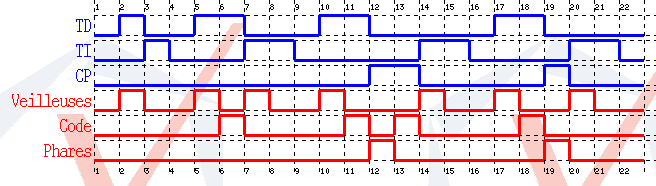
\includegraphics[scale=0.5]{img/chrono1_feux.png}
        \caption{Chronogramme du contrôleur de feux de voiture}
        \label{fig:chrono1_feux}
      \end{figure}

  \section{Contrôleur de feux, version étendue}
    \subsection{Analyse et modélisation}
      %% Analyse des spécifications

      Il est demandé d'analyser un système de contrôle de feux de
      voiture similaire au précédent, étendu de quelques
      fonctionnalitées. Les actions modifiant l'état du système sont
      désormais réalisées via une manette et des boutons. L'état du
      système défini l'état des feux de la voiture. \medskip

      Il est spécifié deux nouvelles entrées :
      \begin{itemize}
        \item {\tt AB}, vrai lorsque le bouton anti-brouillard est pressé
        \item {\tt LP}, vrai lorsque le bouton longue-portée est pressé
      \end{itemize} \vspace{1em}

%     Il y a une exclusion mutuelle entre les deux nouvelles entrées. \medskip

      Il est spécifié deux nouvelles sorties :
      \begin{itemize}
        \item {\tt AntiBrouillard}, indique que les anti-brouillards sont allumées
        \item {\tt LonguePortee}, indique que les longue-portées sont allumées
      \end{itemize} \vspace{1em}

      Il y a une exclusion mutuelle entre les deux nouvelles
      sorties. En effet, les anti-brouillards ne peuvent être allumés que
      lorsque les codes sont allumés et les longue-portées ne peuvent
      être allumés que lorsque les phares sont allumés. Or, il y a une
      exclusion mutuelle entre l'allumage des codes et des
      phares. \medskip

      %% Automate
      Il resulte de l'analyse précédente la modélisation du problème
      sous la forme d'un automate (cf. figure \ref{fig:autom_feux-ext}). Les
      trainsitions $td$, $ti$, $cp$, $ab$ et $lp$
      correspondent au passage des entrées {\tt TD}, {\tt TI}, {\tt
        CP}, {\tt AB} et {\tt LP} respectivement, à la valeur {\tt
        true}.

      \paragraph{État de l'automate}
        \begin{itemize}
          \item[$q_0$] Aucun feux n'est allumé
          \item[$q_1$] Les veilleuses sont allumées
          \item[$q_2$] Les codes sont allumés
          \item[$q_3$] Les phares sont allumés
          \item[$q_4$] Les codes et les anti-brouillards sont allumés
          \item[$q_5$] Les phares et les longue-portées sont allumés
        \end{itemize}

      \begin{figure}
        \centering
        \begin{tikzpicture}[->,>=stealth',shorten >=1pt,auto,node
            distance=2.8cm,semithick]
          
          \node[state,initial] (A) at ( 0,  1) {$q_0$};
          \node[state]         (B) at ( 0, -2) {$q_1$};
          \node[state]         (C) at (-2, -5) {$q_2$};
          \node[state]         (D) at ( 2, -5) {$q_3$};
          \node[state]         (E) at (-4, -2) {$q_4$};
          \node[state]         (F) at ( 4, -2) {$q_5$};

          \path (A) edge [bend left] node {$td$} (B)
                (B) edge [bend left] node {$ti$} (A)
                    edge             node {$td$} (C)
                (C) edge [bend left] node {$ti$} (B)
                    edge             node {$cp$} (D)
                    edge [bend left] node {$ab$} (E)
                (D) edge             node {$ti$} (B)
                    edge [bend left] node {$cp$} (C)
                    edge             node {$lp$} (F)
                (E) edge             node {$ti$} (B)
                    edge             node {$ab$} (C)
                (F) edge             node {$ti$} (B)
                    edge [bend left] node {$lp$} (D);
        \end{tikzpicture}
        \caption{Automate du contrôleur de feux étendu}
        \label{fig:autom_feux-ext}
      \end{figure}

    \subsection{Simulation et vérification}
      %% Simulations commentées

      Il est demandé de réaliser une simulation d'execution de notre automate
      afin de valider un ensemble de cas de tests simples (cf. figures
      \ref{fig:chrono1_feux-ext} et \ref{fig:chrono2_feux-ext}). Les différents
      cas commencent par un pas d'execution avec l'ensemble des entrées à la
      valeur {\tt false}.

      \paragraph{Premier cas}
        \begin{itemize}
          \item Le signal {\tt TD} est émis, ce qui allume les veilleuses
          \item Le signal {\tt TD} est émis, ce qui éteint les veilleuses et
            allume les codes
          \item Le signal {\tt AB} est émis, ce qui allume les anti-brouillards
          \item Le signal {\tt AB} est émis, ce qui éteint les anti-brouillards
          \item Le signal {\tt TI} est émis, ce qui éteint les codes et allume
            les veilleuses
          \item Le signal {\tt TI} est émis, ce qui éteint les veilleuses
        \end{itemize}

      \paragraph{Second cas}
        \begin{itemize}
          \item Le signal {\tt TD} est émis, ce qui allume les veilleuses
          \item Le signal {\tt TD} est émis, ce qui éteint les veilleuses et
            allume les codes
          \item Le signal {\tt AB} est émis, ce qui allume les anti-brouillards
          \item Le signal {\tt TI} est émis, ce qui éteint les codes ainsi que
            les anti-brouillards et allume les veilleuses
          \item Le signal {\tt TI} est émis, ce qui éteint les veilleuses
        \end{itemize}

      \begin{figure}
        \centering
        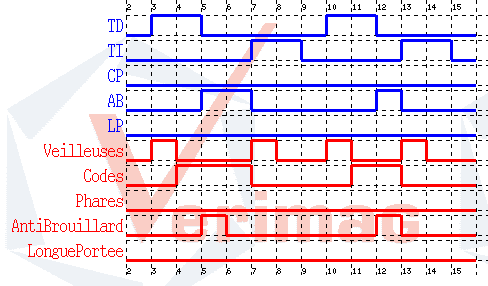
\includegraphics[scale=0.5]{img/chrono1_feux-ext.png}
        \caption{Chronogramme du contrôleur de feux étendu -- Feux anti-brouillard}
        \label{fig:chrono1_feux-ext}
      \end{figure}

      \paragraph{Troisième cas}
        \begin{itemize}
          \item Le signal {\tt TD} est émis, ce qui allume les veilleuses
          \item Le signal {\tt TD} est émis, ce qui éteint les veilleuses et
            allume les codes
          \item Le signal {\tt CP} est émis, ce qui éteint les codes et allume
            les phares 
          \item Le signal {\tt LP} est émis, ce qui allume les longue-portées
          \item Le signal {\tt LP} est émis, ce qui éteint les longue-portées
          \item Le signal {\tt CP} est émis, ce qui éteint les phares et allume
            les codes 
          \item Le signal {\tt TI} est émis, ce qui éteint les codes et allume
            les veilleuses
          \item Le signal {\tt TI} est émis, ce qui éteint les veilleuses
        \end{itemize}

      \paragraph{Quatrième cas}
        \begin{itemize}
          \item Le signal {\tt TD} est émis, ce qui allume les veilleuses
          \item Le signal {\tt TD} est émis, ce qui éteint les veilleuses et
            allume les codes
          \item Le signal {\tt CP} est émis, ce qui éteint les codes et allume
            les phares 
          \item Le signal {\tt LP} est émis, ce qui allume les longue-portées
          \item Le signal {\tt TI} est émis, ce qui éteint les phares ainsi que
            les longue-portées et allume les veilleuses
          \item Le signal {\tt TI} est émis, ce qui éteint les veilleuses
        \end{itemize} \medskip

      \begin{figure}
        \centering
        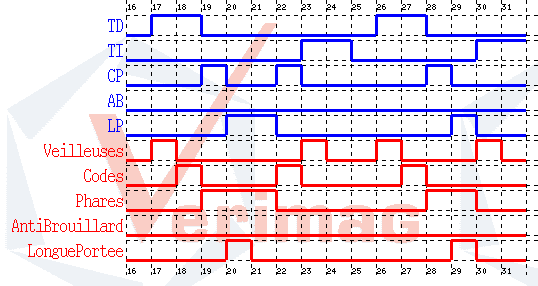
\includegraphics[scale=0.5]{img/chrono2_feux-ext.png}
        \caption{Chronogramme du contrôleur de feux étendu -- feux longue-portées}
        \label{fig:chrono2_feux-ext}
      \end{figure}

      %% Propriétés et vérifications
      Il est demandé de vérifier formellement un certain nombre de propriètés du
      système. Ces vérifications ont été validées grace à l'outil {\tt xlesar}. 

      \paragraph{Première propriété}
        \begin{itemize}
          \item[] Il y a exclusion mutuelle entre les sorties {\tt Veilleuses}, {\tt Codes}
            et {\tt Phares}.
          \item[] \noindent
            {\tt Veilleuses} $\implies$ $\lnot$ ({\tt Codes} $\lor$ {\tt Phares}) \newline
            {\tt Codes} $\implies$ $\lnot$ ({\tt Phares} $\lor$ {\tt Veilleuses}) \newline
            {\tt Phares} $\implies$ $\lnot$ ({\tt Veilleuses} $\lor$ {\tt Codes}) \medskip
        \end{itemize}

      \paragraph{Seconde propriété}
        \begin{itemize}
          \item[] Les anti-brouillards ne peuvent être allumés que si les codes
            sont allumés.
          \item[] \noindent
            {\tt AntiBrouillard} $\implies$ {\tt Codes}
        \end{itemize}

      \paragraph{Troisième propriété}
        \begin{itemize}
          \item[] Les longue-portées ne peuvent être allumés que si les phares
            sont allumés.
          \item[] \noindent
            {\tt LonguePortee} $\implies$ {\tt Phares}
        \end{itemize}

  \section{Contrôleur de porte de tramway}
    \subsection{Analyse et modélisation}

      Il est demandé d'analyser un système de contrôle de porte de tramway. Les
      actions modifiant l'état du système sont réalisées par un tramway, une
      porte de tramway ainsi qu'un utilisateur. L'état du système défini l'état
      de la porte du tramway. \medskip

      %% Analyse des spécifications
      Il est spécifié quatres entrèes :
      \begin{itemize}
        \item {\tt en\_station}, vrai lorsque le tramway est à quai
        \item {\tt attention\_depart}, vrai lorsque le ramassage des passagers
          est terminé
        \item {\tt demande\_porte}, vrai lorsqu'un utilisateur presse le bouton
          d'ouverture de la porte de tramway
        \item {\tt porte\_ouverte}, vrai lorsque la porte de tramway est ouverte
      \end{itemize} \vspace{1em}

      Il y a des contraintes sur l'état initial de certaines entrée. En effet,
      il est précisé que les entrées {\tt en\_station} et {\tt porte\_ouverte}
      doivent être fixées à la valeur {\tt false} initialement. \medskip

      Il est spécifié sept sorties :
      \begin{itemize}
        \item {\tt depart}, vrai lorsque le tramway quitte le quais
        \item {\tt depart\_imminent}, vrai lorsque le tramway a émis {\tt
          attention\_depart} 
        \item {\tt accepter\_demande}, vrai lorsqu'une demande d'ouverture peut
          être prise en compte
        \item {\tt porte\_demandee}, vrai lorsqu'une demande d'ouverture a été
          accéptée 
        \item {\tt ouvrir\_porte}, vrai lorsque la porte est en cours d'ouverture
        \item {\tt fermer\_porte}, vrai lorsque la porte est en cours de fermeture
        \item {\tt porte\_ok}, vrai lorsque la porte se ferme
      \end{itemize} \vspace{1em}

      Plusieurs hypothèses ont été avancées concernant l'environement du
      contrôleur de porte de tramway.
      \begin{itemize}
        \item Le tramway ne peut quitter un station qu'une fois le signal {\tt
          attention\_depart} émit par ce dernier
        \item Le tramway ne peut quitter une station qu'une fois le signal {\tt
          porte\_ok} émit par le contrôleur
        \item La porte ne peut être ouverte ou fermée que si le contôleur a émit
          le signal {\tt ourvir\_porte} ou {\tt fermer\_porte} respectivement
      \end{itemize} \vspace{1em}

      %% Automate

      Il résulte de l'analyse précédente la modélisation du problème sous la
      forme d'un automate (cf. figure \ref{fig:autom_tram}).  Les evenements sur
      les transistions correspondent à de front descendant ou montant sur les
      entrèes associées selon si elles sont précédées ou non du symbole de
      négation $\lnot$, respectivement.  Les actions sur les transitions
      correspondent au passage des sorties associées aux valeurs {\tt false} ou
      {\tt true} selon si elles sont précédées ou non du symbole de négation
      $\lnot$, respectivement.

      \paragraph{État de l'automate}
        \begin{itemize}
          \item[$q_0$] Le tramway est en transit entre deux stations
          \item[$q_1$] Le tramway est en transit entre deux station et une
            demande d'ouverture de la porte a été prise en compte
          \item[$q_2$] Le tramway est à quais et il n'y a pas de demande
            d'ouverture de la porte
          \item[$q_3$] La porte est en cours d'ouverture
          \item[$q_4$] La porte est ouverte
          \item[$q_5$] La porte est en cours de fermeture
          \item[$q_6$] Le tramway peut repartir
        \end{itemize}

      \paragraph{Transitions de l'automate}
        \begin{itemize}
          \item[$a$] {\tt demande\_porte / porte\_demandee}
          \item[$b$] {\tt en\_station /}
          \item[$c$] {\tt en\_station / ouvrir\_porte}
          \item[$d$] {\tt demande\_porte / porte\_demandee; ouvrir\_porte}
          \item[$e$] {\tt porte\_ouverte / $\lnot$ ourvir\_porte}
          \item[$f$] {\tt attention\_depart / depart\_imminent; $\lnot$
            accepter\_demande; fermer\_porte}
          \item[$g$] {\tt $\lnot$ porte\_ouverte / $\lnot$ fermer\_porte; porte\_ok}
          \item[$h$] {\tt $\lnot$ en\_station / depart; accepter\_demande}
          \item[$i$] {\tt attention\_depart / depart\_imminent; $\lnot$
            accepter\_demande; porte\_ok}
        \end{itemize}

      \begin{figure}
        \centering
        \begin{tikzpicture}[->,>=stealth',shorten >=1pt,auto,node
            distance=2.8cm,semithick] 
          
          \node[state,initial] (A) at ( 0,  0) {$q_0$};
          \node[state]         (B) at ( 3, -2) {$q_1$};
          \node[state]         (C) at ( 3,  2) {$q_2$};
          \node[state]         (D) at ( 6,  0) {$q_3$};
          \node[state]         (E) at ( 6,  4) {$q_4$};
          \node[state]         (F) at ( 3,  6) {$q_5$};
          \node[state]         (G) at ( 0,  4) {$q_6$};
          
          \path (A) edge node [below] {$a$} (B)
                    edge node         {$b$} (C)
                (B) edge node [below] {$c$} (D)
                (C) edge node         {$d$} (D)
                    edge node         {$i$} (G)
                (D) edge node [right] {$e$} (E)
                (E) edge node [above] {$f$} (F)
                (F) edge node [above] {$g$} (G)
                (G) edge node [left ] {$h$} (A);
        \end{tikzpicture}
        \caption{Automate du contrôleur de porte de tramway}
        \label{fig:autom_tram}
      \end{figure}

    \subsection{Simulation et vérification}
      %% Simulations commentées
    
      Il est demandé de réaliser une simulation d'execution de notre automate
      afin de valider un ensemble de cas de testes simples (cf. figure
      \ref{fig:chrono1_tram}). Les différents cas commencent par un pas
      d'execution avec l'ensemble de entrées à la valeur {\tt
        false}. Initialement {\tt accepter\_demande} a la valeur {\tt true}.

      \paragraph{Premier cas}
        \begin{itemize}
          \item Le signal {\tt en\_station} est émis
          \item Le signal {\tt attention\_depart} est émis, ce qui désacive {\tt
            accepter\_demande} et active {\tt depart\_imminent} et {\tt
            porte\_ok}
          \item Le signal $\lnot$ {\tt en\_station} est émis, ce qui desactive
            {\tt depart\_imminent} et active {\tt depart} et {\tt
              accepter\_demande} 
        \end{itemize}

      \paragraph{Deuxième cas}
        \begin{itemize}
          \item Le signal {\tt en\_station} est émis
          \item Le signal {\tt demande\_porte} est émis, ce qui active {\tt
            porte\_demande} et {\tt ourvir\_porte}
          \item Le signal {\tt porte\_ouverte} est émis, ce qui désactive {\tt
            ourvir\_porte} 
          \item Le signal {\tt attention\_depart} est émis, ce qui désacive {\tt
            accepter\_demande} et active {\tt depart\_imminent} et {\tt
            fermer\_porte}
          \item Le signal $\lnot$ {\tt porte\_ouverte} est émis, ce qui
            désactive {\tt fermer\_porte} et active {\tt porte\_ok}
          \item Le signal $\lnot$ {\tt en\_station} est émis, ce qui desactive
            {\tt depart\_imminent} et active {\tt depart} et {\tt
              accepter\_demande} 
        \end{itemize}

      \paragraph{Troisième cas}
        \begin{itemize}
          \item Le signal {\tt demande\_porte} est émis, ce qui active {\tt
            porte\_demande}
          \item Le signal {\tt en\_station} est émis, ce qui active {\tt
            ourvir\_porte}
          \item Le signal {\tt porte\_ouverte} est émis, ce qui désactive {\tt
            ourvir\_porte}
          \item Le signal {\tt attention\_depart} est émis, ce qui désacive {\tt
            accepter\_demande} et active {\tt depart\_imminent} et {\tt
            fermer\_porte}
          \item Le signal $\lnot$ {\tt porte\_ouverte} est émis, ce qui
            désactive {\tt fermer\_porte} et active {\tt porte\_ok}
          \item Le signal $\lnot$ {\tt en\_station} est émis, ce qui desactive
            {\tt depart\_imminent} et active {\tt depart} et {\tt
              accepter\_demande} 
        \end{itemize}

      \begin{figure}
        \centering
        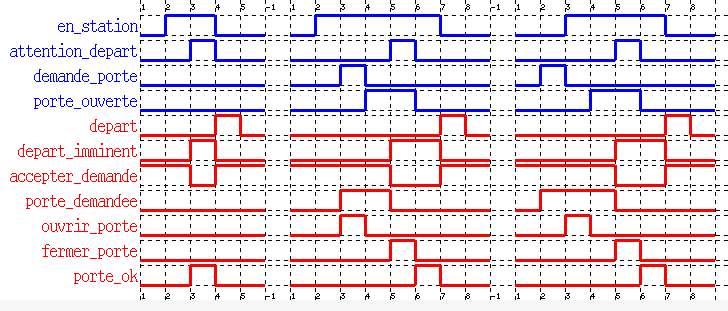
\includegraphics[scale=0.5]{img/chrono1_tram.png}
        \caption{Chronogramme du contrôleur de porte de tramway}
        \label{fig:chrono1_tram}
      \end{figure}

      %% Propriétés et vérifications
      \medskip
      Il est demandé de vérifier formellement une proprièté du
      système. Cette vérification a été validée grace à l'outil {\tt xlesar}.

      \paragraph{Propriété}
        \begin{itemize}
          \item[] Le tramway ne peut jamais rouler avec la porte ouverte.
          \item[] \noindent
            $\lnot$ {\tt en\_station} $\implies$ $\lnot$ {\tt porte\_ouverte} \medskip
        \end{itemize}

  \appendix
  \section{Fichiers sources}
    \subsection{Contrôleur de feux de voiture}
      \begin{lstlisting}
node FEUX (TD, TI, CP: bool)
returns (Veilleuses, Codes, Phares: bool);
var Eteint: bool;
let

  -- Preconditon: Only one input in {TD, TI, CP} is true simultaneously. 
  assert not (TD and TI);
  assert not (TI and CP);
  assert not (CP and TD);

  Eteint = not TD ->
    if TI and pre Veilleuses then true else
    if TD and pre Eteint then false else
    pre Eteint;

  Veilleuses = TD ->
    if TD and pre Eteint then true else
    if TI and (pre Codes or pre Phares) then true else
    if TD and pre Veilleuses then false else
    if TI and pre Veilleuses then false else
    pre Veilleuses;

  Codes = false ->
    if TD and pre Veilleuses then true else
    if CP and pre Phares then true else
    if TI and pre Codes then false else
    if CP and pre Codes then false else
    pre Codes;

  Phares = false ->
    if CP and pre Codes then true else
    if TI and pre Phares then false else
    if CP and pre Phares then false else
    pre Phares;
tel
      \end{lstlisting}    

    \subsection{Contrôleur de feux étendu}
      \begin{lstlisting}
node FEUX (TD, TI, CP, AB, LP: bool)
returns (Veilleuses, Codes, Phares, AntiBrouillard, LonguePortee: bool);
var Eteint: bool;
let
  
  -- Preconditon: Only one input in {TD, TI, CP} is true simultaneously. 
  assert not (TD and TI);
  assert not (TI and CP);
  assert not (CP and TD);

  -- Preconditon: Only one input in {AB, LP} is true simultaneously. 
  assert not (AB and LP);

  Eteint = not TD ->
    if TI and pre Veilleuses then true else
    if TD and pre Eteint then false else
    pre Eteint;
    
  Veilleuses = TD ->
    if TD and pre Eteint then true else
    if TI and (pre Codes or pre Phares) then true else
    if TD and pre Veilleuses then false else
    if TI and pre Veilleuses then false else
    pre Veilleuses;

  Codes = false ->
    if TD and pre Veilleuses then true else
    if CP and pre Phares then true else
    if TI and pre Codes then false else
    if CP and pre Codes then false else
    pre Codes;

  Phares = false ->
    if CP and pre Codes then true else
    if TI and pre Phares then false else
    if CP and pre Phares then false else
    pre Phares;
 
  AntiBrouillard = false ->
    Codes and (if AB and not pre AntiBrouillard then true else
               if AB and pre AntiBrouillard then false else
               pre AntiBrouillard);

  LonguePortee = false ->
    Phares and (if LP and not pre LonguePortee then true else
                if LP and pre LonguePortee then false else
                pre LonguePortee);

  -- Postcondition: Only one output in {Veilleuses, Codes, Phares} is
  --   true simultaneously.
  -- Veilleuses => not (Codes      or Phares)
  -- Codes      => not (Phares     or Veilleuses)
  -- Phares     => not (Veilleuses or Codes)

  -- Postcondition: AntiBrouillard implies Codes and LonguePortee
  --   implies Phares.
  -- AntiBrouillard => Codes
  -- LonguePortee   => Phares

tel
      \end{lstlisting}
    
    \subsection{Contrôleur de porte de tramway}
      \begin{lstlisting}
node TRAM (en_station, attention_depart, demande_porte, porte_ouverte: bool)
returns (depart, depart_imminent, accepter_demande, porte_demandee,
         ouvrir_porte, fermer_porte, porte_ok: bool);
let

  -- Hypothesis on the tramway:
  --  The tramway is initially not in station
  --  Leaving a station implies door is OK
  assert (not (en_station) -> true);
  assert (ONCE_FROM_TO (RISING_EDGE (en_station),
          FALLING_EDGE (en_station),
          attention_depart));

  assert (ONCE_FROM_TO (attention_depart,
          FALLING_EDGE (en_station),
          porte_ok));

  --  Emitting departure signal implies being in station and not opening the door
  assert (attention_depart => en_station and
                              not (pre (ouvrir_porte)));

  -- Hypothesis on the door:
  --  The door is initially closed
  --  The door becoming open implies that it was previously opening
  --  The door becoming closed implies that it was previously closing 
  assert (not (porte_ouverte) -> true);
  assert (RISING_EDGE  (porte_ouverte) => pre ouvrir_porte);
  assert (FALLING_EDGE (porte_ouverte) => pre fermer_porte);

  depart = FALLING_EDGE (en_station);
  depart_imminent = false ->
    (attention_depart or pre (depart_imminent))
    and not (depart);

  accepter_demande = true ->
    (depart or pre (accepter_demande))
    and not (RISING_EDGE (depart_imminent));

  porte_demandee = demande_porte ->
    (demande_porte or pre (porte_demandee))
    and accepter_demande;

  ouvrir_porte = en_station and not (depart_imminent)
                 and porte_demandee and not (porte_ouverte);

  fermer_porte = en_station and depart_imminent and porte_ouverte;
  porte_ok = en_station and depart_imminent
             and not (porte_ouverte);

  -- Postcondition: The tramway never move with the door open
  -- not (en_station) => not (porte_ouverte)

tel
      \end{lstlisting}      

\end{document}
